\documentclass[12pt]{article}

\newlength\tindent
\setlength{\tindent}{\parindent}
\setlength{\parindent}{0pt}
\renewcommand{\indent}{\hspace*{\tindent}}

%% packages
\usepackage{enumerate}
\usepackage{listings}
\usepackage{amsmath}
\usepackage{multicol}
\usepackage{caption}
\usepackage{subcaption}
\usepackage[a4paper,margin=2cm]{geometry}
% \usepackage[english, norsk]{babel}
\usepackage{fancyhdr}
\usepackage{pdfpages}
\usepackage{lastpage}
% \usepackage[demo]{graphicx}
\usepackage{graphicx}
\usepackage{placeins}
\graphicspath{ {.} }

%Framed image panel
\newcommand\FramedImage[2][]{%
  \setlength\fboxsep{1pt}% change according to needs
  \setlength\fboxrule{3pt}%
  \noindent\fbox{%
    \begin{minipage}[c][\dimexpr.3\textheight-1.5\fboxrule-2\fboxsep\relax][c]{\dimexpr.5\textwidth-1.5\fboxrule-2\fboxsep\relax}
    \centering
    \includegraphics[#1]{#2}
  \end{minipage}}%
}
\newcommand{\FIXME}[1]{{\bfseries FIXME: #1}}
\newcommand{\COMMENT}[2]{{\bfseries COMMENT~(#1): #2}}
\date{}
\begin{document}

% intentionally empty
%\author{Faculty of Mathematics and Natural Sciences}

\title{Additional exercises}

\maketitle 

This paper consists of \pageref{LastPage} pages including appendices. \\
Permitted materials: calculator

\section{Random variable parameter estimation}

A discrete random variable $X$ is defined by
  \begin{equation}
    X=
    \begin{cases}
      -20, & prob.=1/3 \\
       30, & prob.=1/2 \\
       10, & prob.=1/6
    \end{cases}
  \end{equation}

\begin{enumerate}[(a)] 
\item find the expected value
\item find the variance
\item find the mode
\item find the coefficient of variation
\end{enumerate}


\section{Probability density function}
The probability density function of a random variable $x$ is given as:

$$ f(x)=\frac{1}{\sqrt{2 \pi \sigma^2}} e^{- \frac{(x-\mu)^2}{2 \sigma^2}} $$

\begin{enumerate}[(a)] 
\item Draw a free-hand figure to illustrate the density function and indicate on the figure the probability $prob(x<a)$, $prob(a<x<b)$ and $prob(x>b)$
\item Draw a free-hand figure to illustrate the cumulative probability distribution function and indicate on the figure the probability $prob(x<a)$,  $prob(a<x<b)$ and $prob(x>b)$.
\item Define or explain the first and second moment of $x$.
\item Explain the 68-95-99.7-percent rule
\end{enumerate}


%\pagebreak
\section{Frequency analysis and linear regression}
\begin{enumerate}[(a)]
\item What is the probability to observe at least one 200-years flood or larger within a period of 10 years?
\item Figure 1A shows a simple linear regression between average runoff and median annual flood. Figure 1B shows the QQ-plot of the residual where the theoretical quantiles were calculated using the normal distribution. Describe which assumption of a simple linear regression is violated in this analysis, and discuss strategies that can be used to improve the analysis.
\end{enumerate}

\begin{figure}[h!]
    \centering
    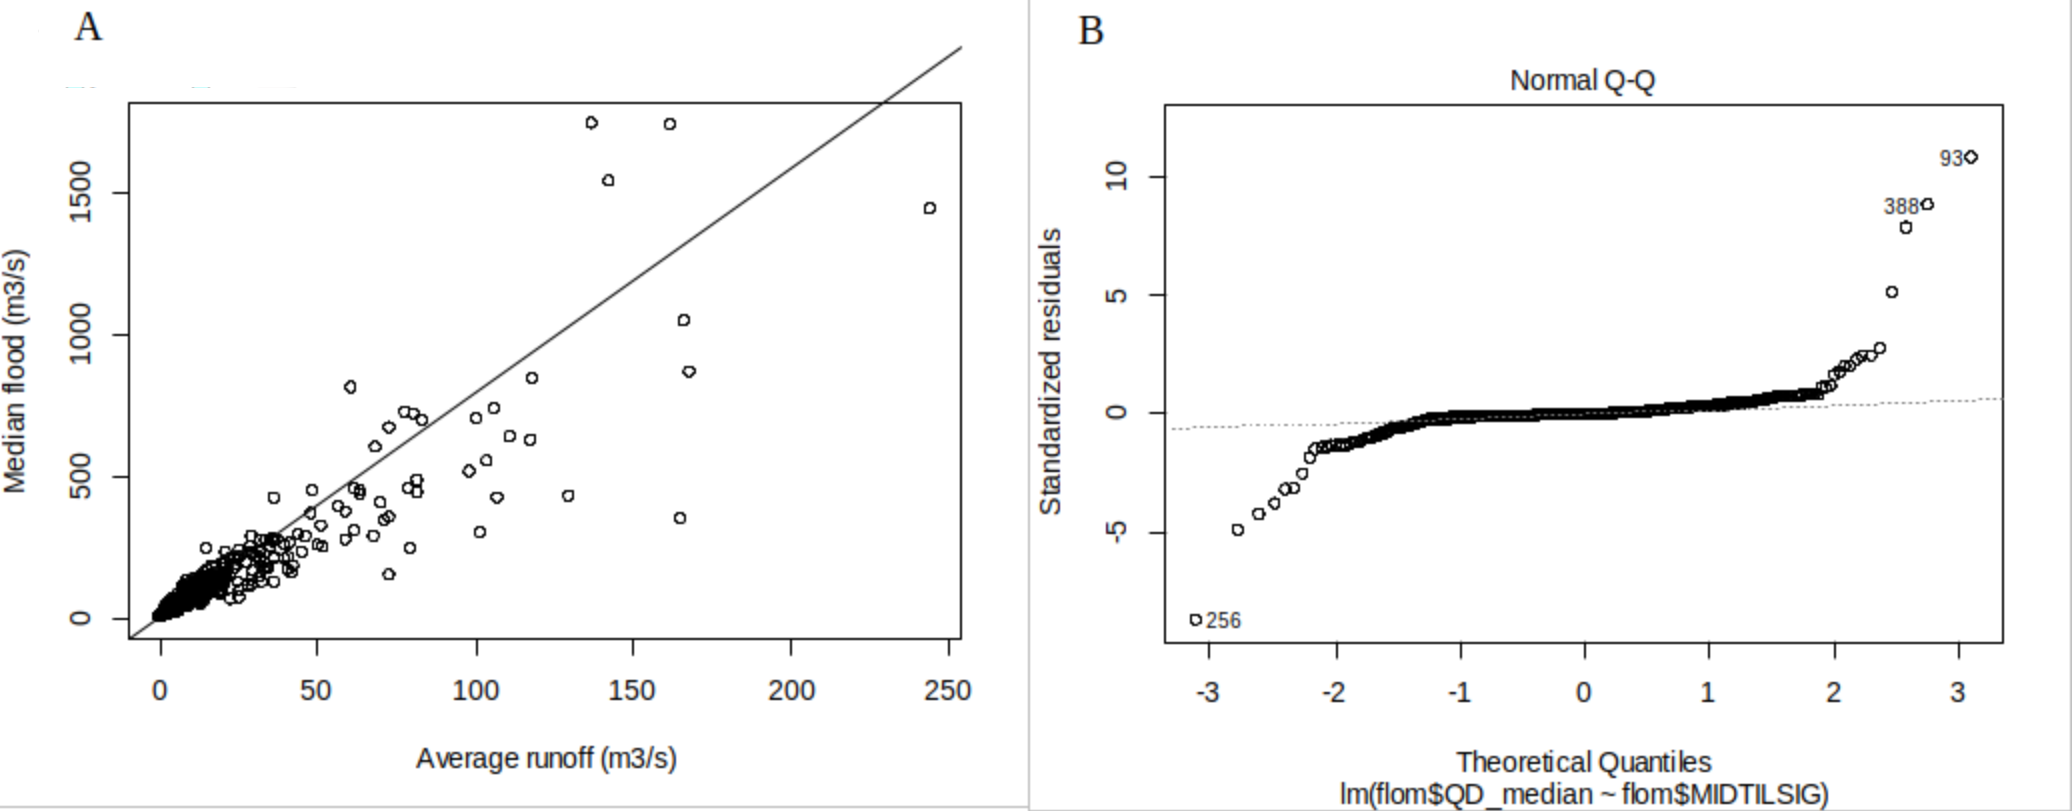
\includegraphics[width=.8\textwidth]{fig01} 
    \caption{A) linear regression, B) Q-Q plot.}
\end{figure}




\section{Correlation}
Consider the following bi-variate sample:
$$X=\{21, 32, 34, 11, 32\}$$
$$Y=\{43, 45, 47, 33, 34\}$$
\begin{enumerate}[(a)] 
\item Calculate the Pearson correlation coefficient of $X$ and $Y$.
\item Calculate the Spearman rank correlation of $X$ and $Y$.
 \end{enumerate}
%>>> import scipy.stats as ss
%>>> ss.spearmanr([21, 32, 34, 11, 32],[43, 45, 47, 33, 34])
%(0.8207826816681234, 0.088587005313543785)
%np.corrcoef([21, 32, 34, 11, 32],[43, 45, 47, 33, 34])
%array([[ 1.        ,  0.55108203],
%       [ 0.55108203,  1.        ]])



\section{Confidence intervals}
A sample of 20 random observations produced a mean of 145 and variance of 30. 
\begin{enumerate}[(a)] 
    \item What is the 95\% confidence interval on the mean assuming a normal distribution if 
    \begin{enumerate}[(i)] 
        \item the true variance is unknown and estimated as 30
        \item the true variance is 30
     \end{enumerate}
    \item What is the reason for the difference of results in part (i) and part (ii)?
    \item What is the 95\% confidence interval on the variance?
\end{enumerate}



%\pagebreak
\section{Hypothesis testing}
Below is a 20-year dataset (all values are in m$^3$/s) with observations of runoff before a human intervention, and a 7-year dataset from after the human intervention in a basin. \\

Before the intervention:\\
24, 12, 48, 17, 14, 28, 11, 13, 31, 34, 34, 12, 48, 14, 28, 17, 11, 13, 31, 24 (mean = 23.2, standard deviation = 11.48)\\

After the intervention:\\
29, 46, 49, 31, 28, 50, 31 (mean = 37.7, standard deviation = 9.32)\\


Could it be stated from this small sample that the runoff (both mean and variance) was affected by the intervention? Use a significance level of 5\%. What is the probability of making a type II error in your decision?




\section{Goodness-of-fit testing}
In order to calculate the design flood, you need to know which probability distribution fits your data best. Based on a 35-year record of yearly maximum discharge data from a river station, the following statistics are calculated (with $n = 35$)

Let $Y = \ln Q$ (natural logarithm)

Average: $\bar{Y}=5.257$ 

Standard deviation: $S_Y = 0.686$

The 35 years data are classified into 5 classes as given in the table below.
\begin{table}[h!!]
\begin{tabular}{l|c}
Class & Observed number \\
\hline
$Q \le 100$ & 5 \\
$100<Q \le 150$ & 9 \\
$150<Q \le 200$ & 7 \\
$200<Q \le 300$ & 6 \\
$Q \ge 300$ & 8 \\
\hline
\end{tabular}
\end{table}


\begin{enumerate}[(a)] 
\item Use Chi square method (with significance level of 5\%) to test if the data are log-normally distributed
\item Could the Kolmogorov-Smirnov test also be used to perform the goodness-of-fit test?
\end{enumerate}


\section{Time series analysis}
A 12-year time series of annual measurements is given as the sequence:\\
110, 88, 51, 64, 39, 23, 10, 10, 6, 5, 10, 3

Perform a trend test of your choice to check if the time series contains a trend. Use a significance level of 5\%.



\section{Machine learning}
\begin{enumerate}[(a)] 
\item Why is it common to split the dataset into a training set and a test set when doing machine learning? In your answer, include in a relevant way the terms “training error” and “test error”
\item In many machine learning algorithms you have a parameter that controls the complexity of the model. Why do we want to control this complexity?
\end{enumerate}


\section{Fourier transformation}
Consider the following time series $X_t$ sampled once per second

\begin{figure}[h!]
    \centering
    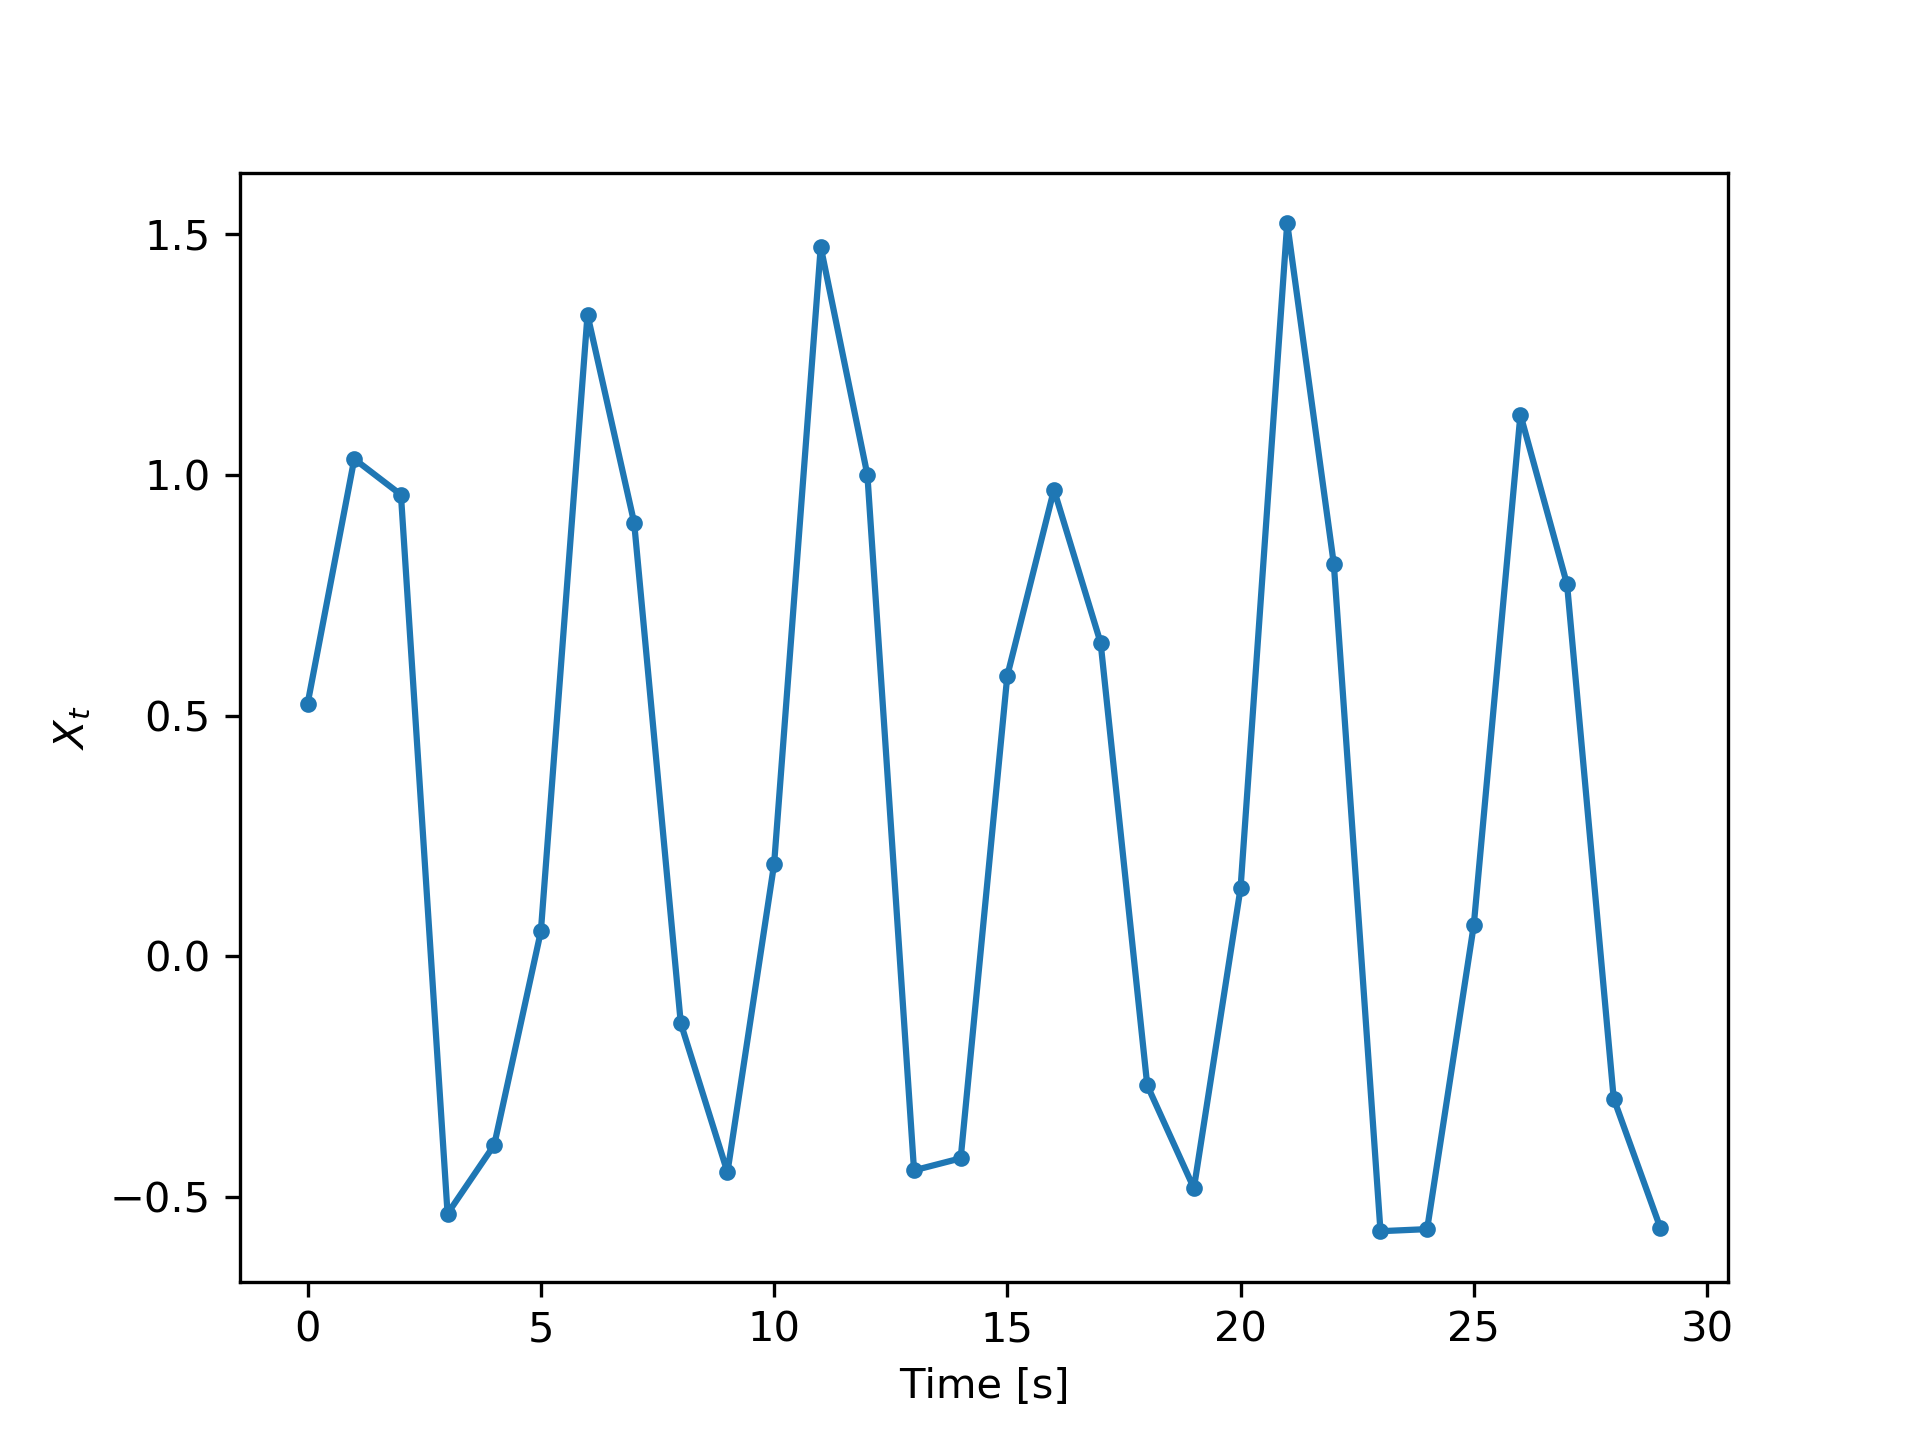
\includegraphics[width=.8\textwidth]{./fourier_figures/Fourier_ts} 
%    \caption{}
\end{figure}

\begin{enumerate}[(a)]
\item The following three graphs show the absolute values for the Fourier coefficients, defined as:
$$ X_k = \sum_{n=0}^{N-1} x_n \cdot e^{-i \, 2 \pi \, k \, n/N} $$

\begin{figure}[h!]
    \centering
    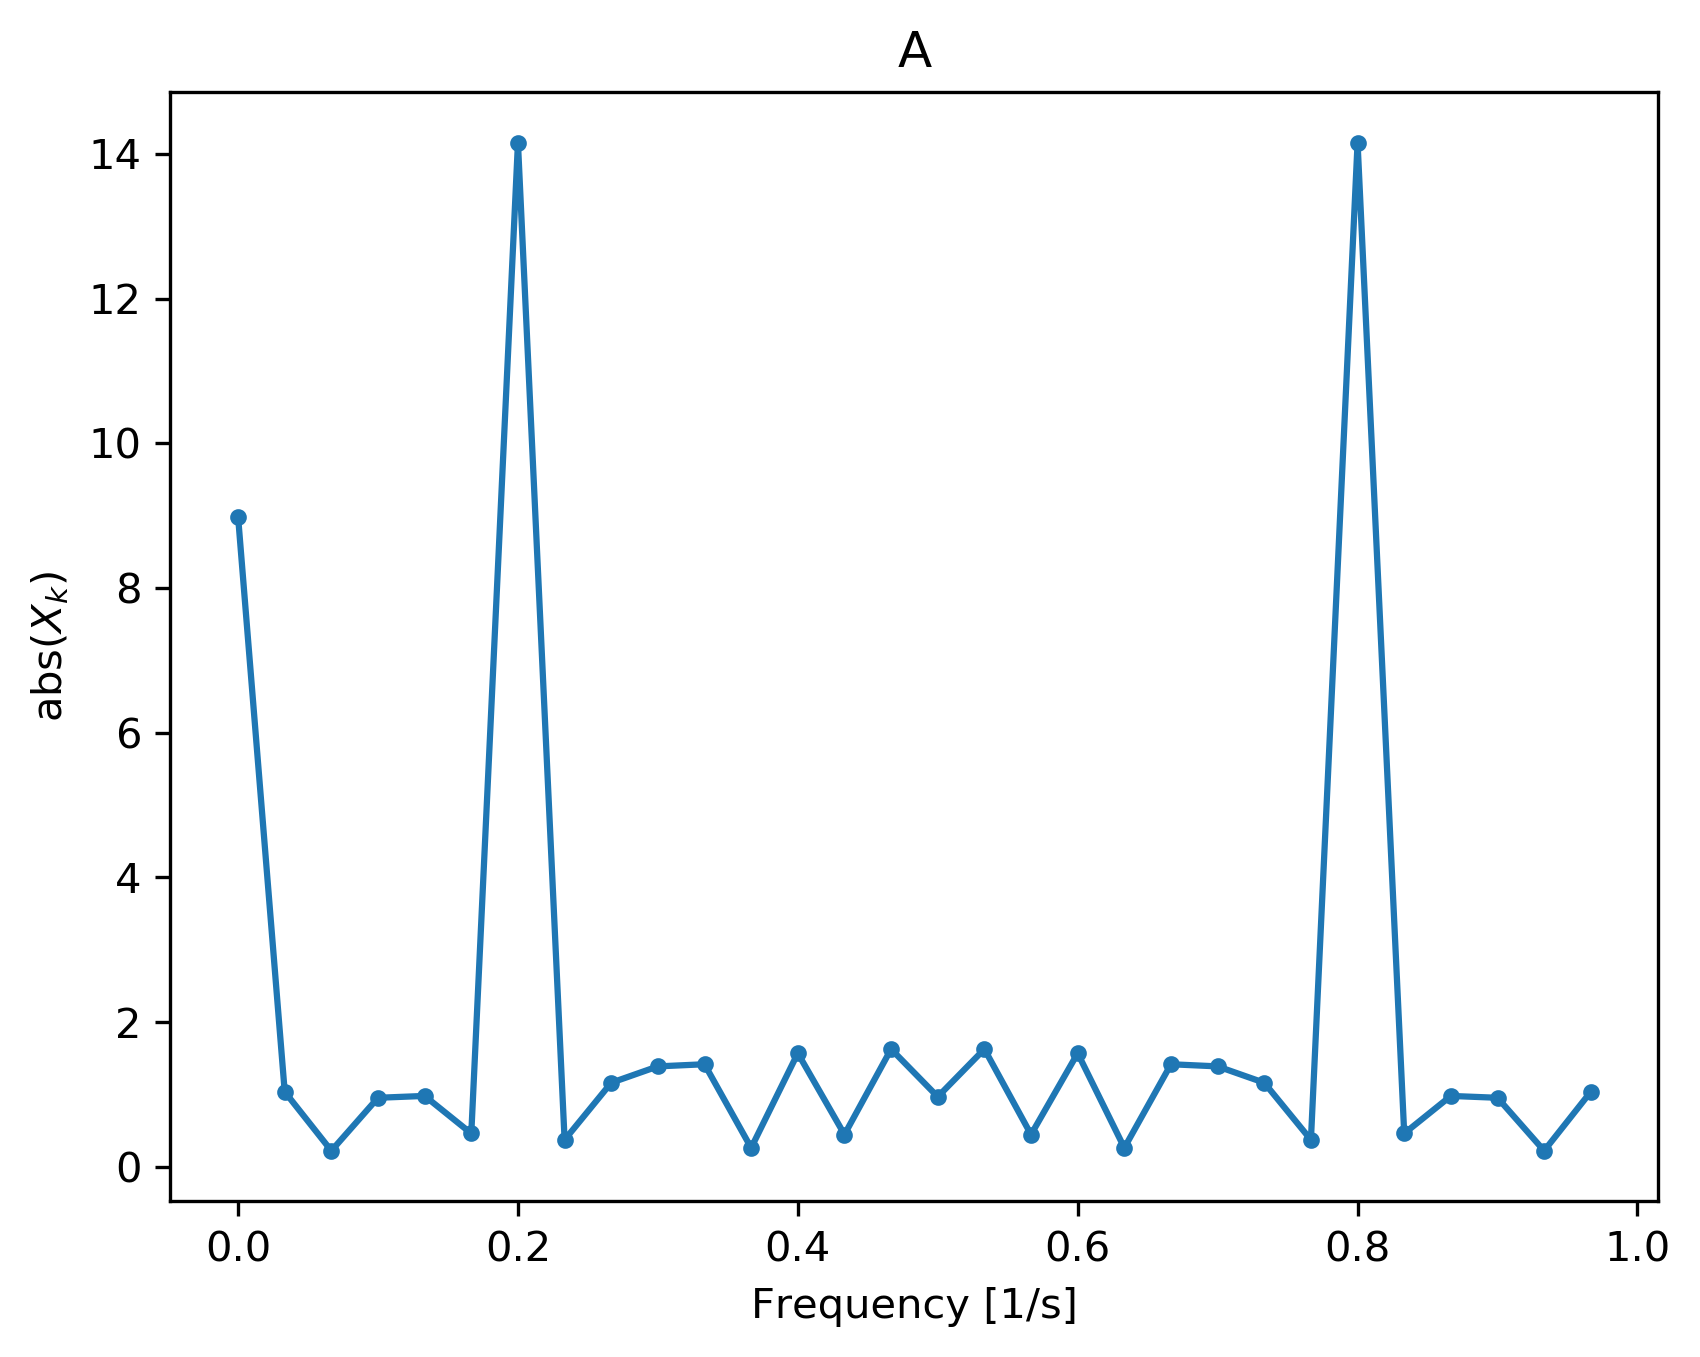
\includegraphics[width=.3\textwidth]{./fourier_figures/Fourier_A}
	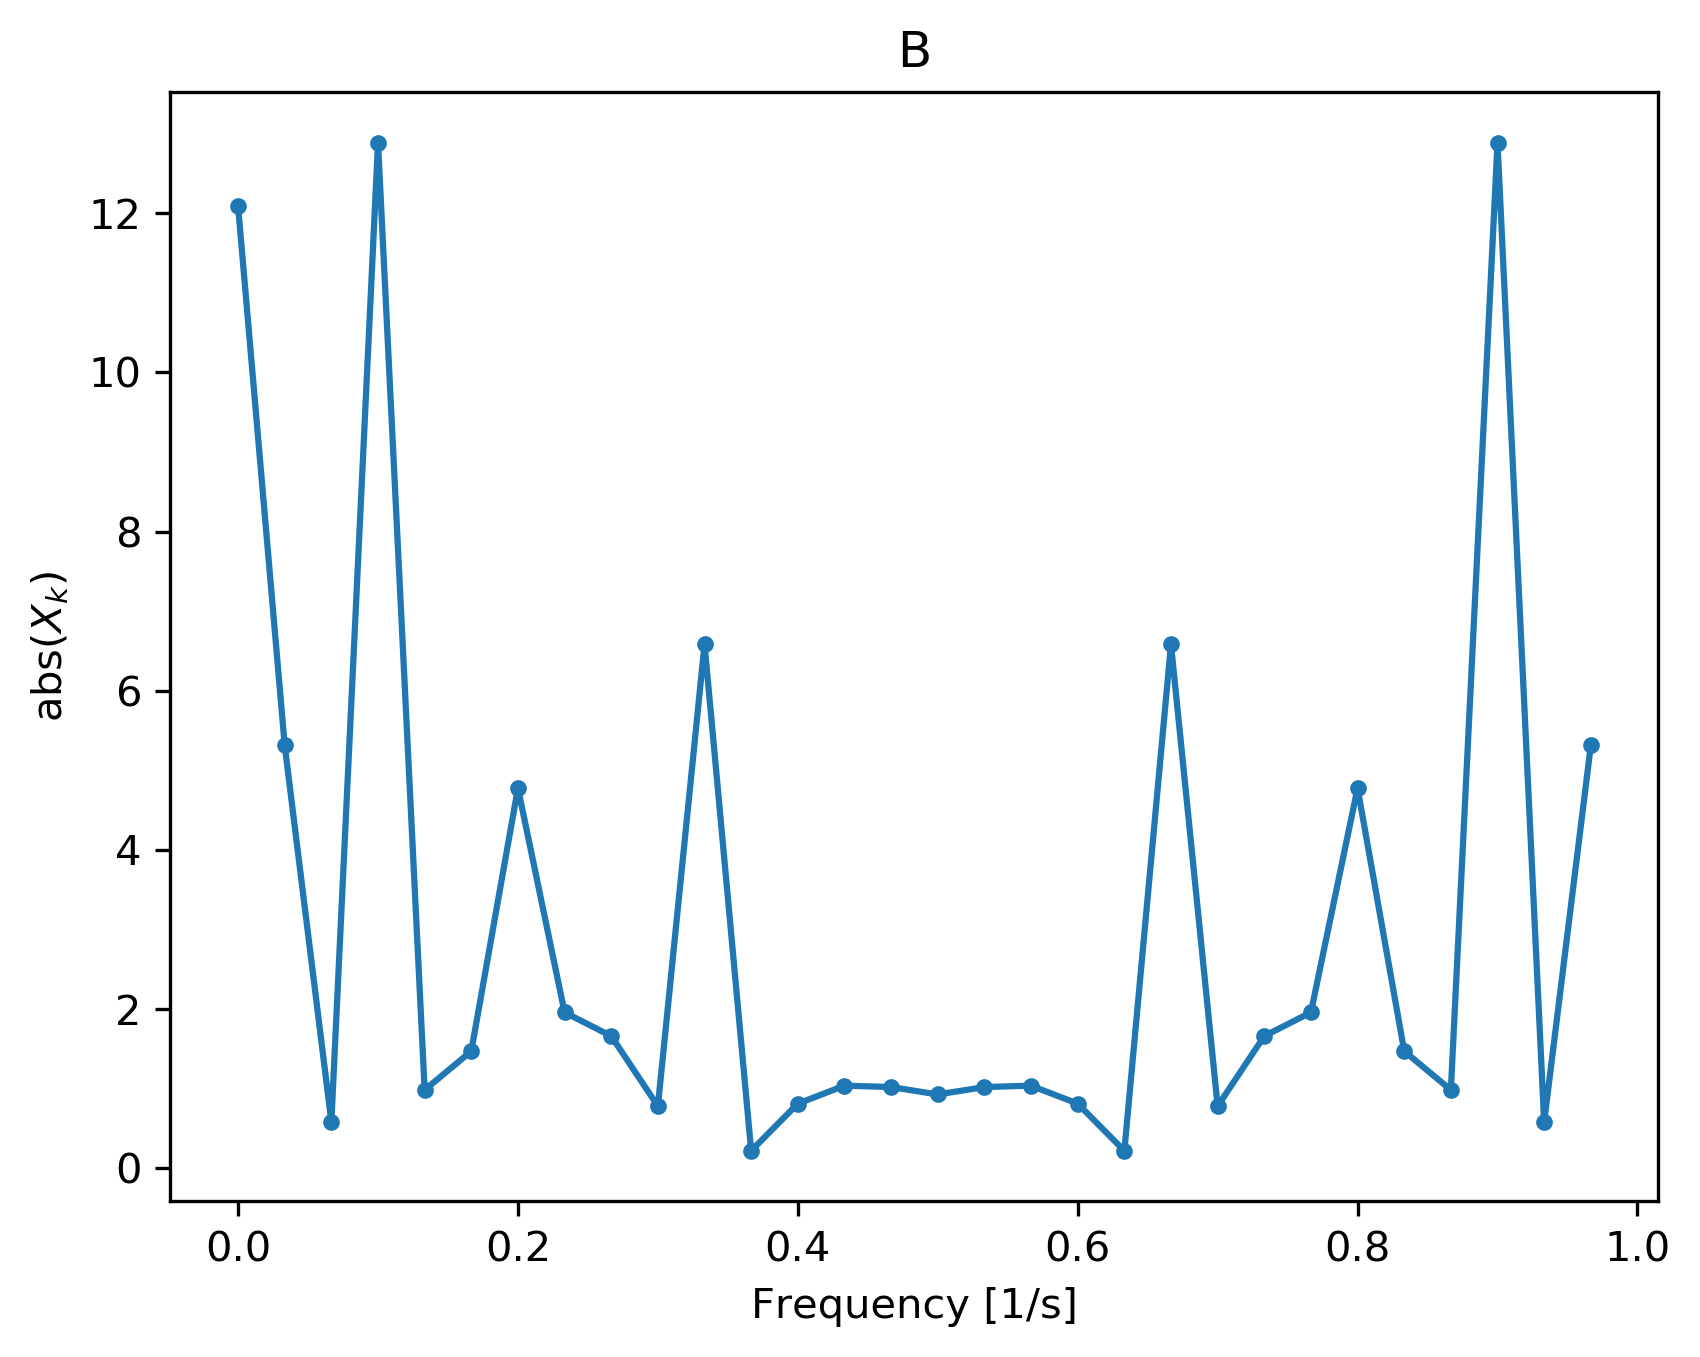
\includegraphics[width=.3\textwidth]{./fourier_figures/Fourier_B}
	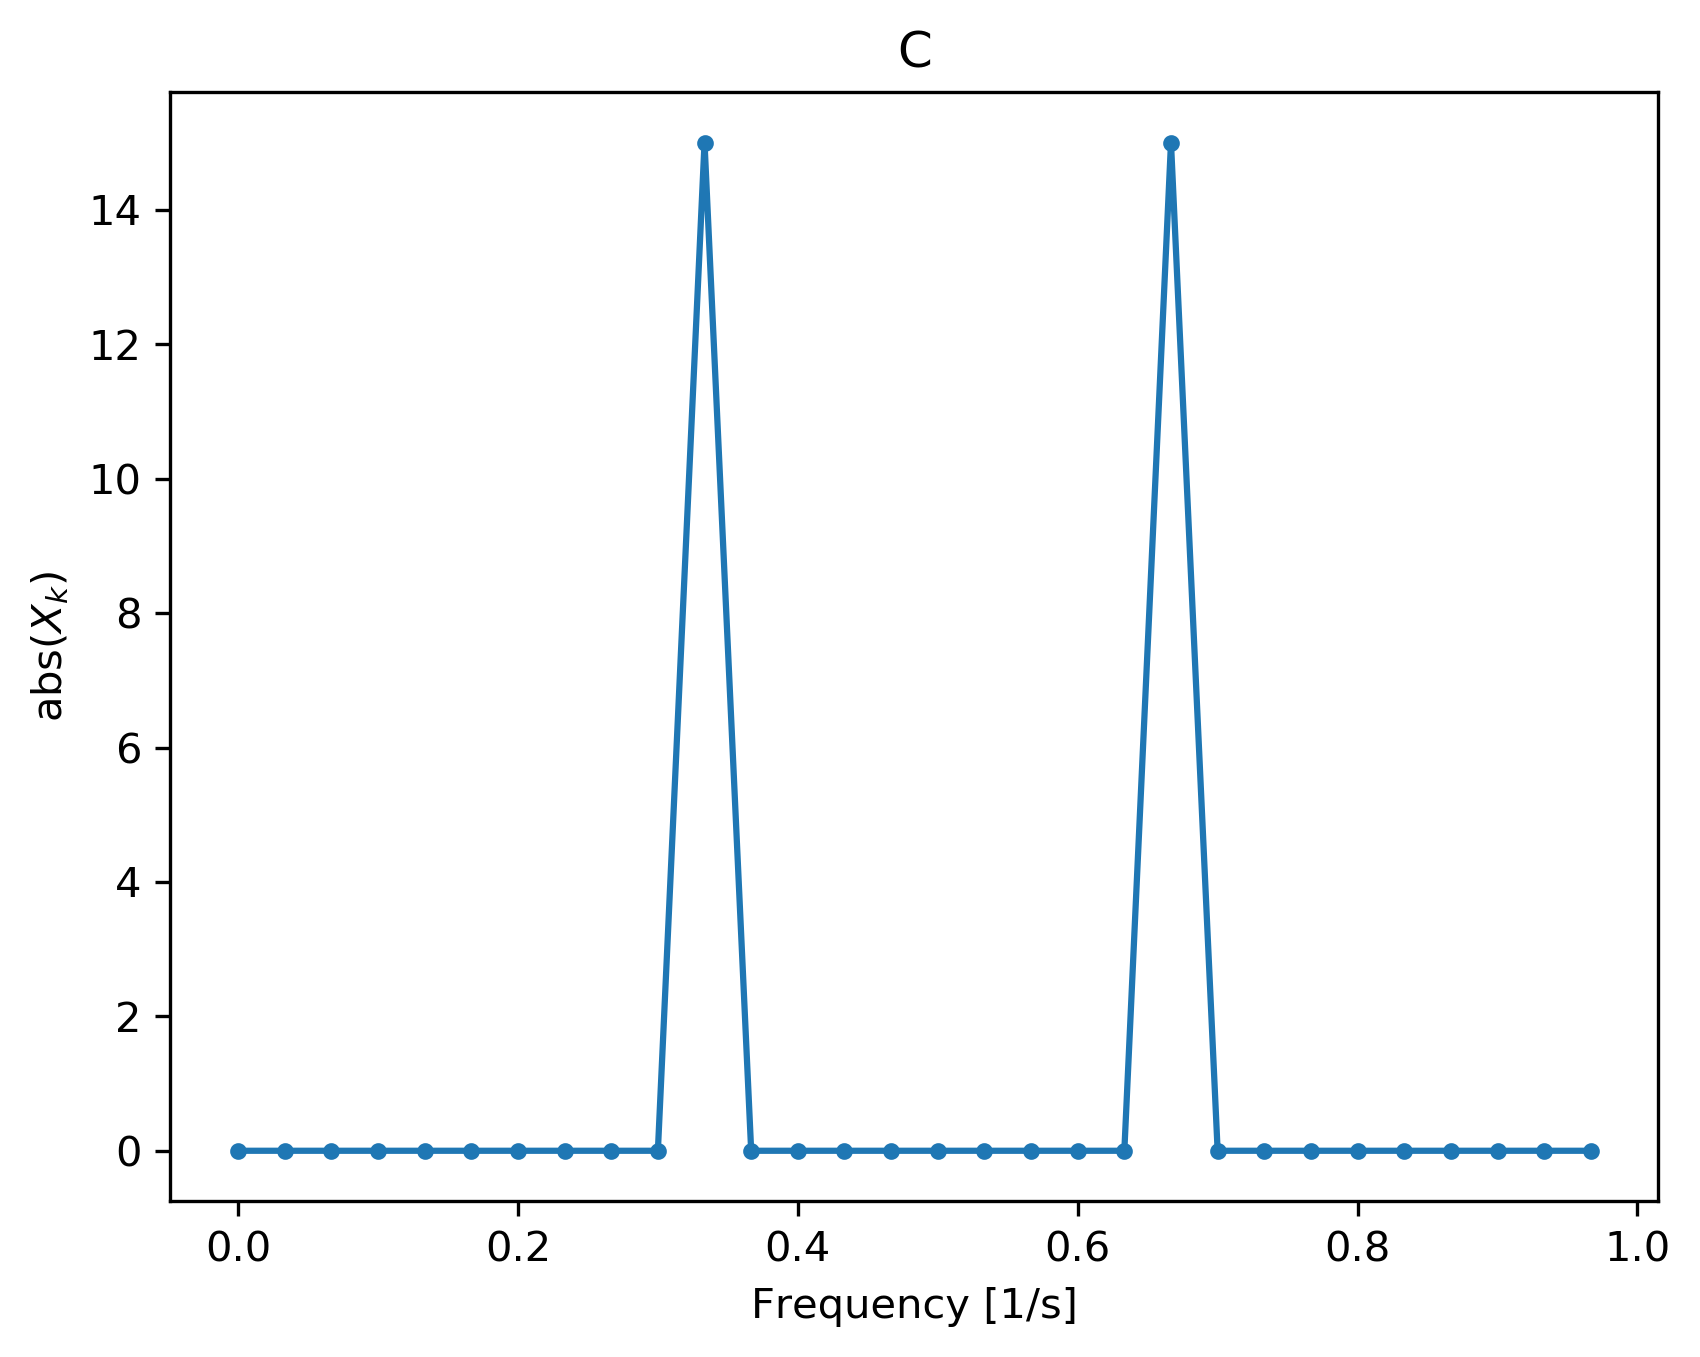
\includegraphics[width=.3\textwidth]{./fourier_figures/Fourier_C} 
%    \caption{}
\end{figure}
Which one of them (A, B or C) shows the Fourier transform of $X_t$? Explain your answer.

\end{enumerate}


\section{Time series analysis and stochastic modeling}
Answer the following statements with True if it is always true, otherwise with False.
\begin{enumerate}[(a)] 
\item Most geoscientific processes (time series) are stochastic processes
\item Stochastic processes (time series) are stationary 
\item An independent time series is a stationary time series 
\item An independent stationary time series is purely random
\item A Gaussian time series is an independent series
\item A Gaussian time series is a stationary time series
\item A white noise times series is normally distributed
\item If Xt is a log-normally distributed time series, then Xt is symmetric about its mean
\item Markov model (i.e. AR(1) model) is used for an independent stationary time series
\item Markov model (i.e. AR(1) model) is used for a nonstationary time series
\end{enumerate}

\pagebreak

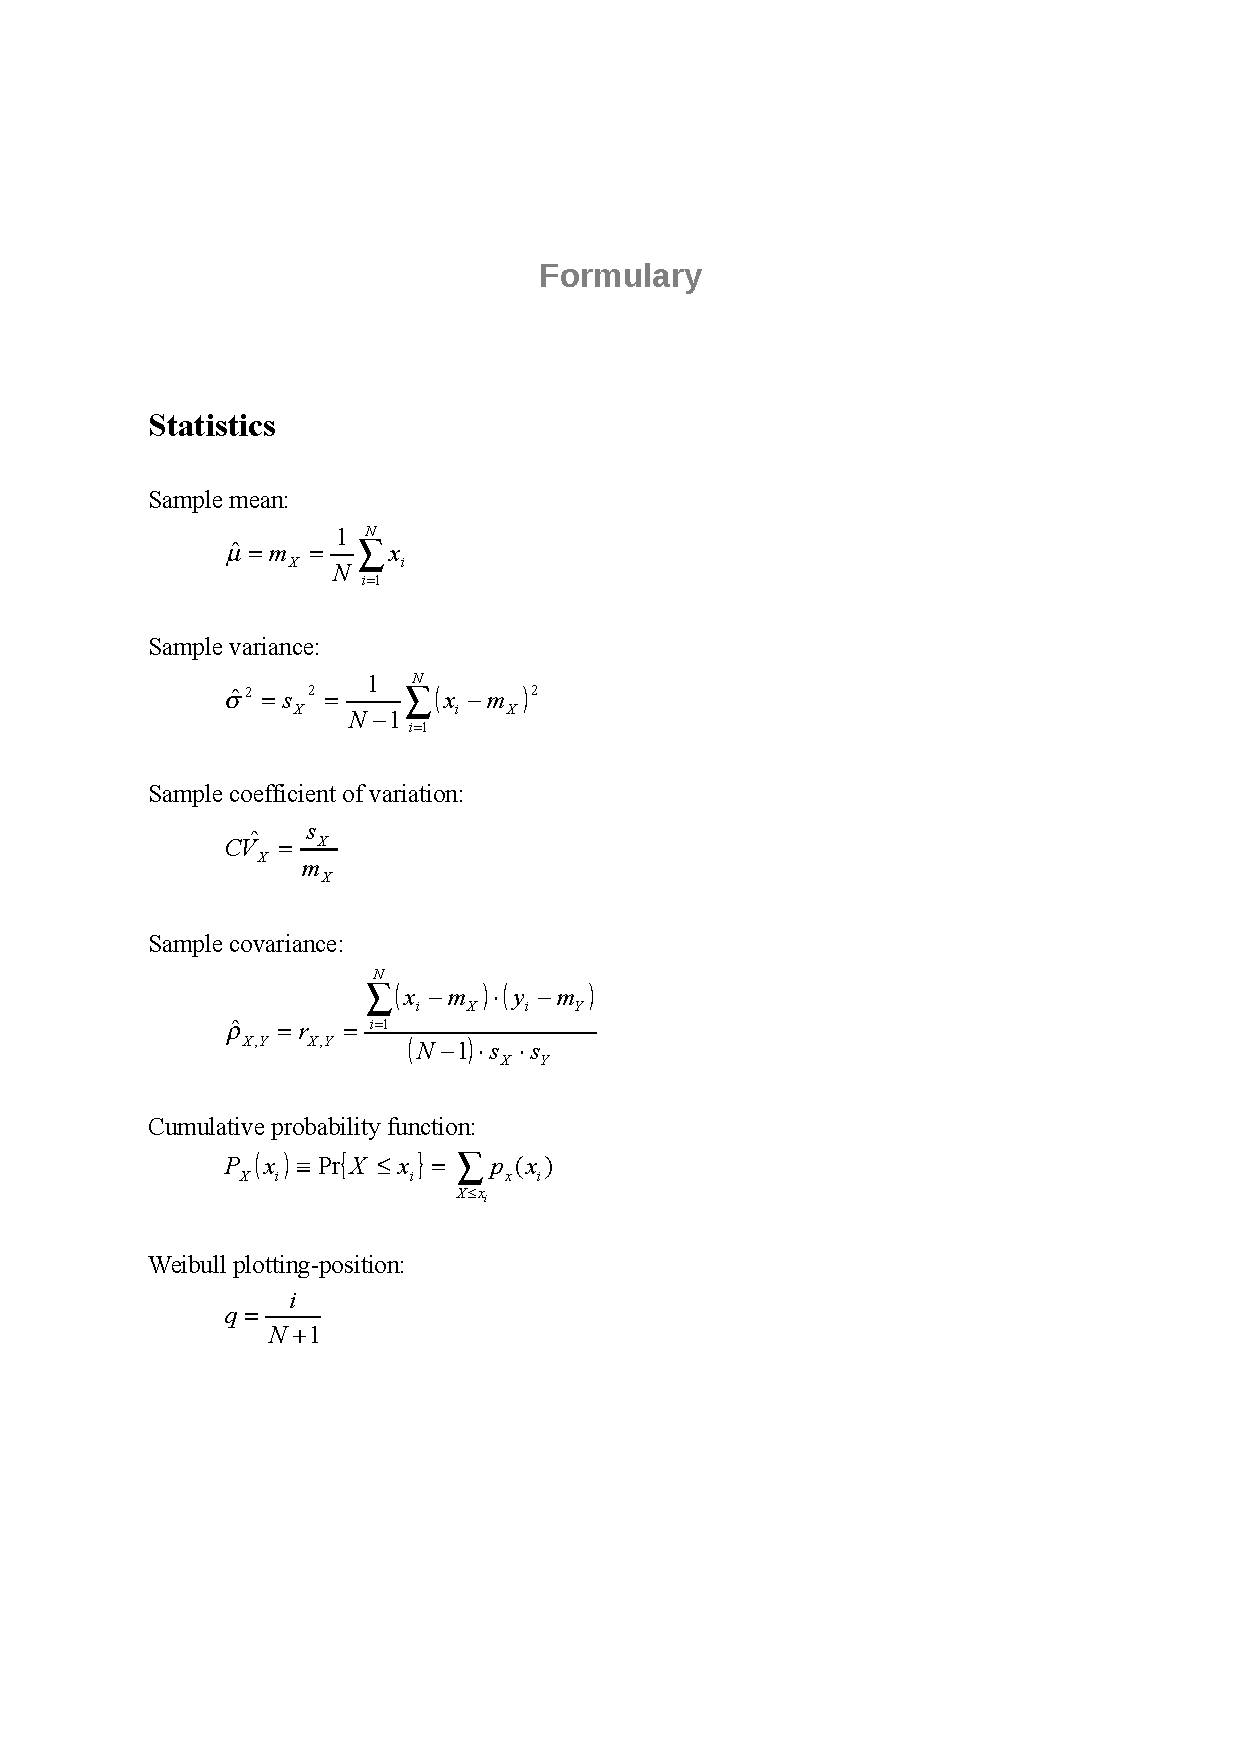
\includepdf[pages={1-12}]{formulary-2017_final.pdf}



\end{document}









